%!TEX root = ../report.tex
\documentclass[../report.tex]{subfiles}

\begin{document}
\section{Manual Motion Observation }
\label{sec:exp01}
The goal of this experiment is to design a differntial drive robot using LEGO EV3 and then measure its pose variation for three different constant velocity motions: an arc to the left, straight line ahead, and an arc to the right.
\subsection{Design of Experiment}

\begin{figure}[ht]
        \centering
        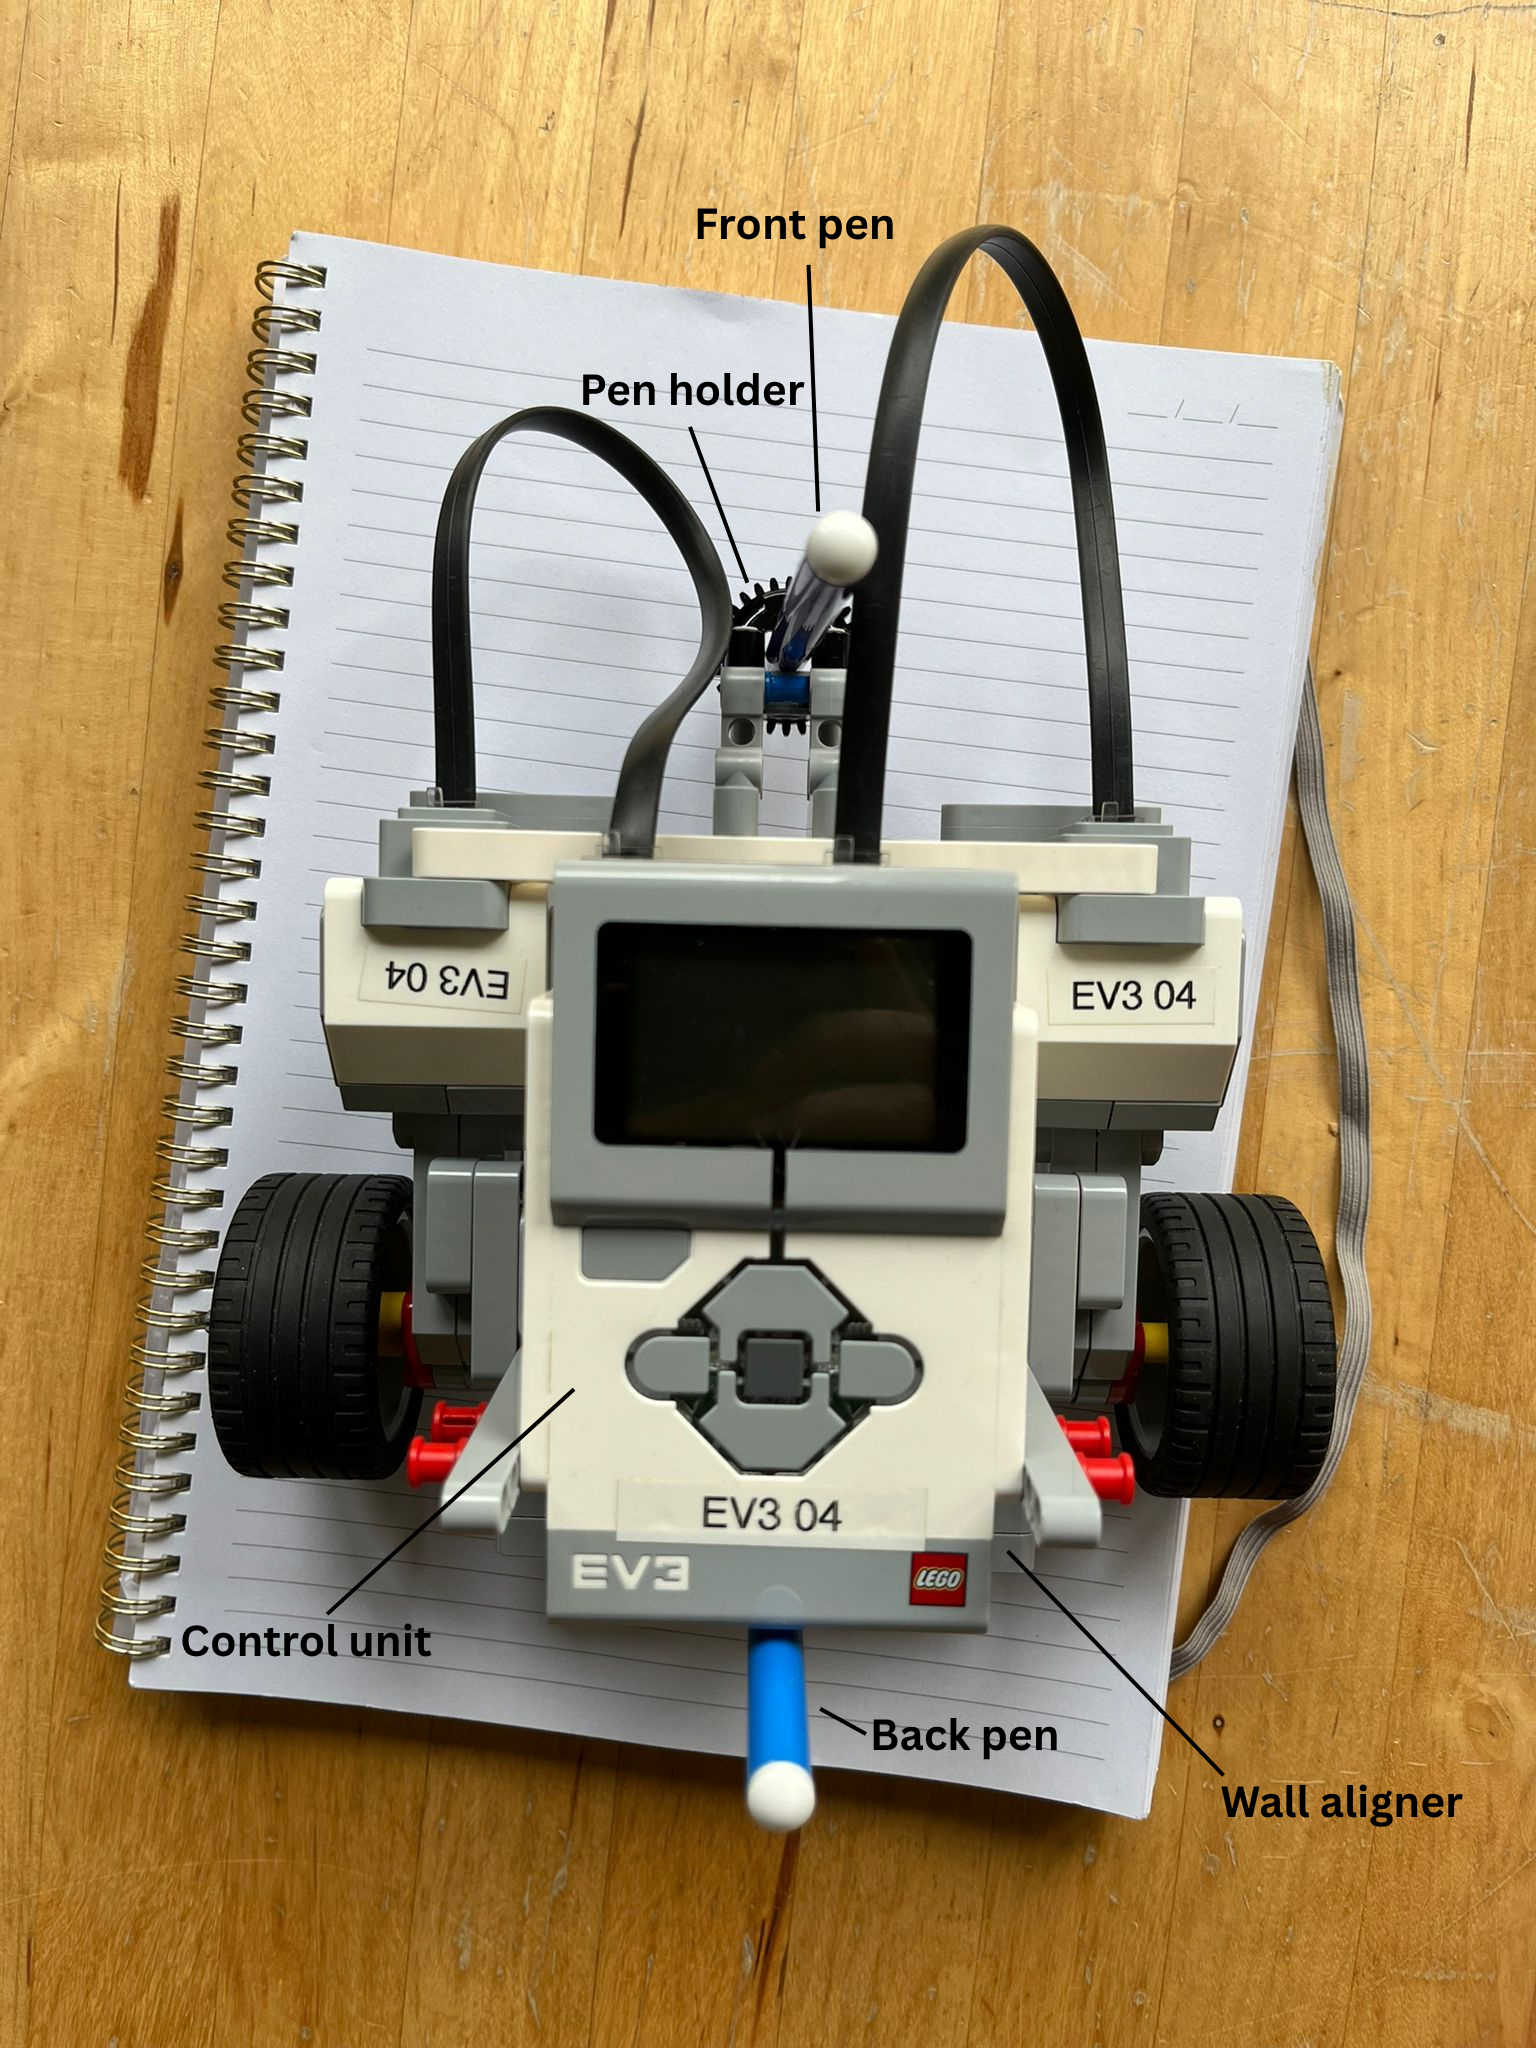
\includegraphics[width=0.8\linewidth]{figures/robot_angles/top.png}
        \caption{Top view of the robot}
        \label{fig:top_view}
    \end{figure}
    
    \begin{figure}[ht]
        \centering
        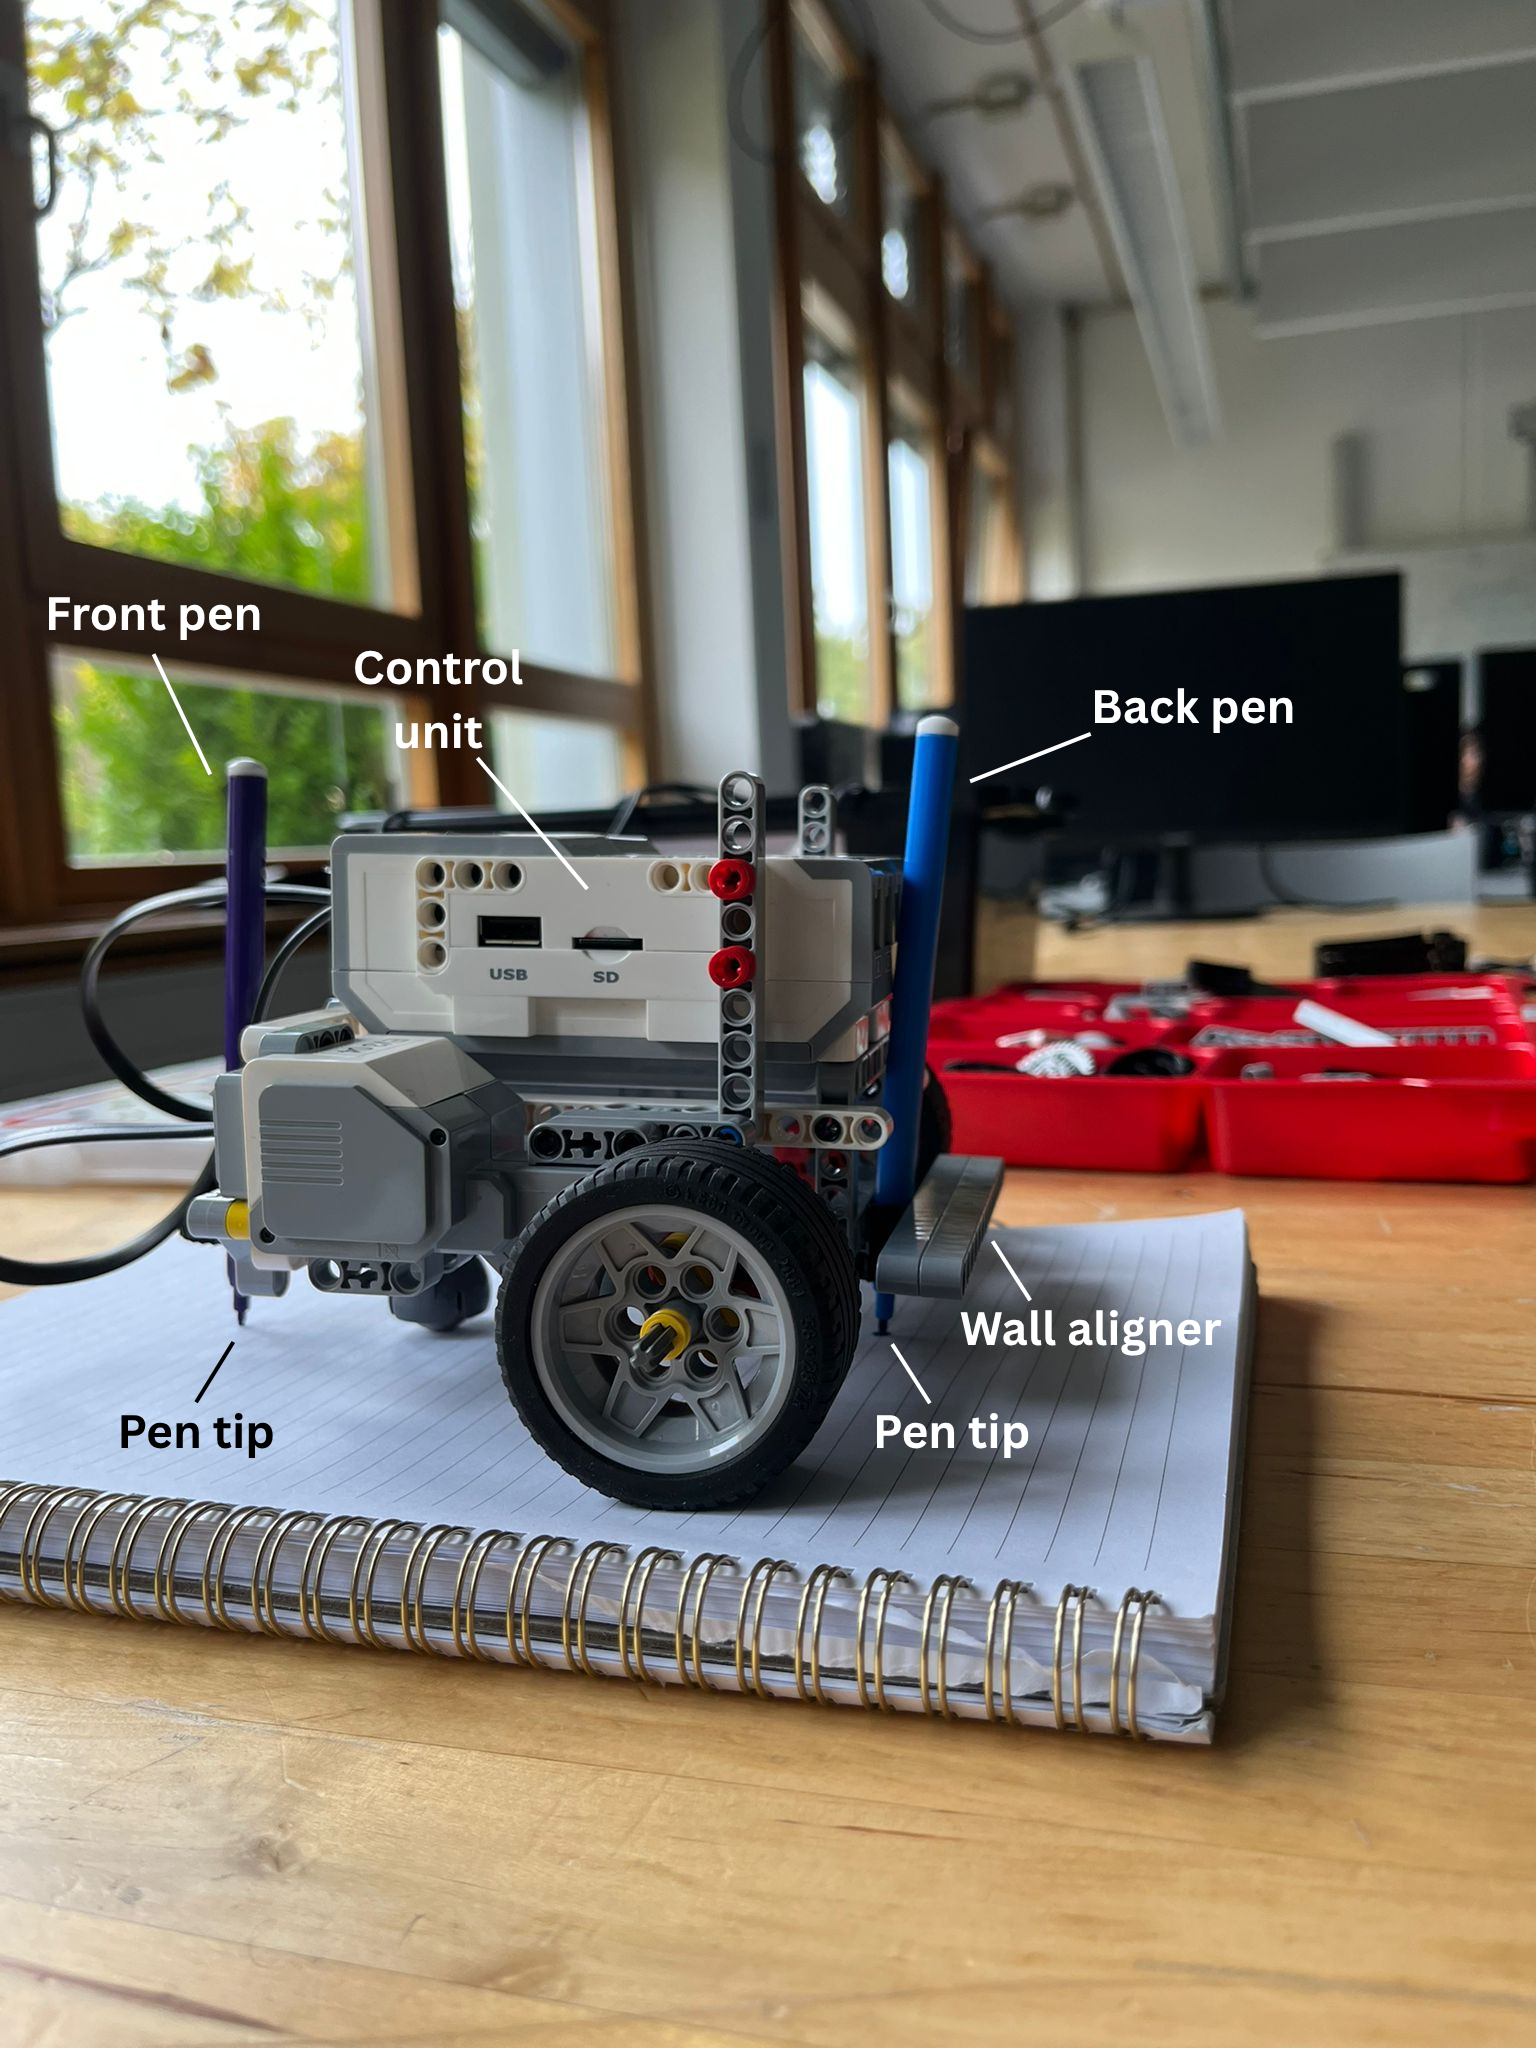
\includegraphics[width=0.8\linewidth]{figures/robot_angles/side.png}
        \caption{Top view of the robot}
        \label{fig:top_view}
    \end{figure}
    
    \begin{figure}[ht]
        \centering
        \includegraphics[width=0.8\linewidth]{figures/robot_angles/front.png}
        \caption{Top view of the robot}
        \label{fig:top_view}
    \end{figure}
    
    \begin{figure}[ht]
        \centering
        \includegraphics[width=0.8\linewidth]{figures/robot_angles/isometric.png}
        \caption{Top view of the robot}
        \label{fig:top_view}
    \end{figure}

    \begin{figure}[ht]
        \centering
        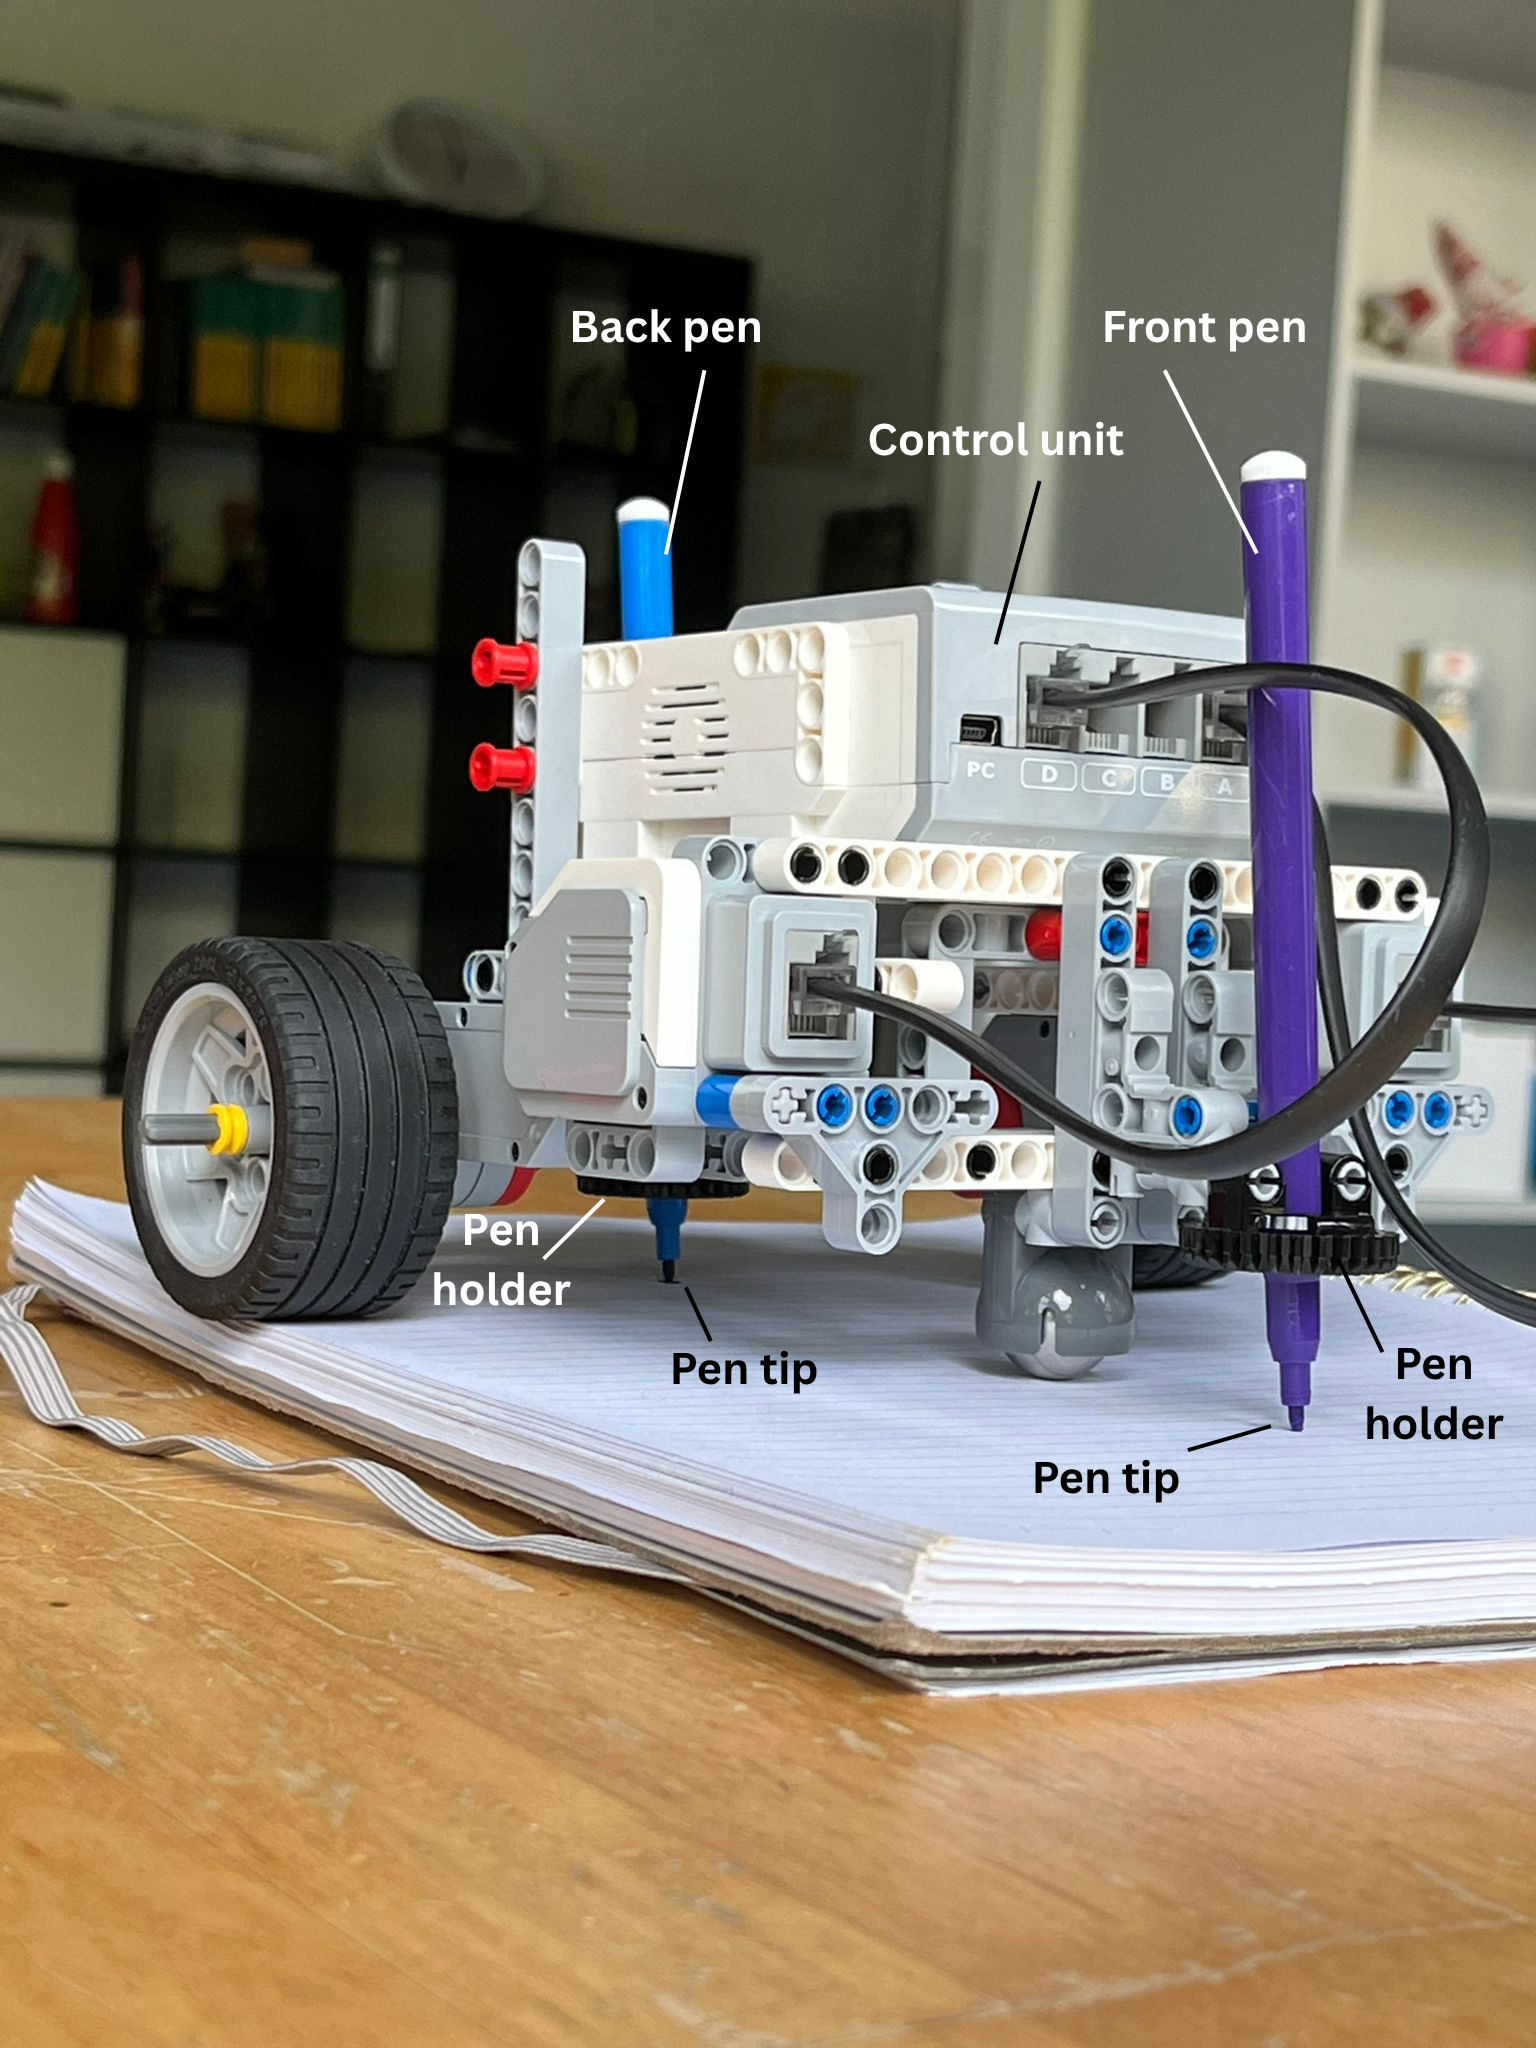
\includegraphics[width=0.8\linewidth]{figures/robot_angles/isometric2.png}
        \caption{Top view of the robot}
        \label{fig:top_view}
    \end{figure}   

    \begin{figure}[ht]
        \centering
        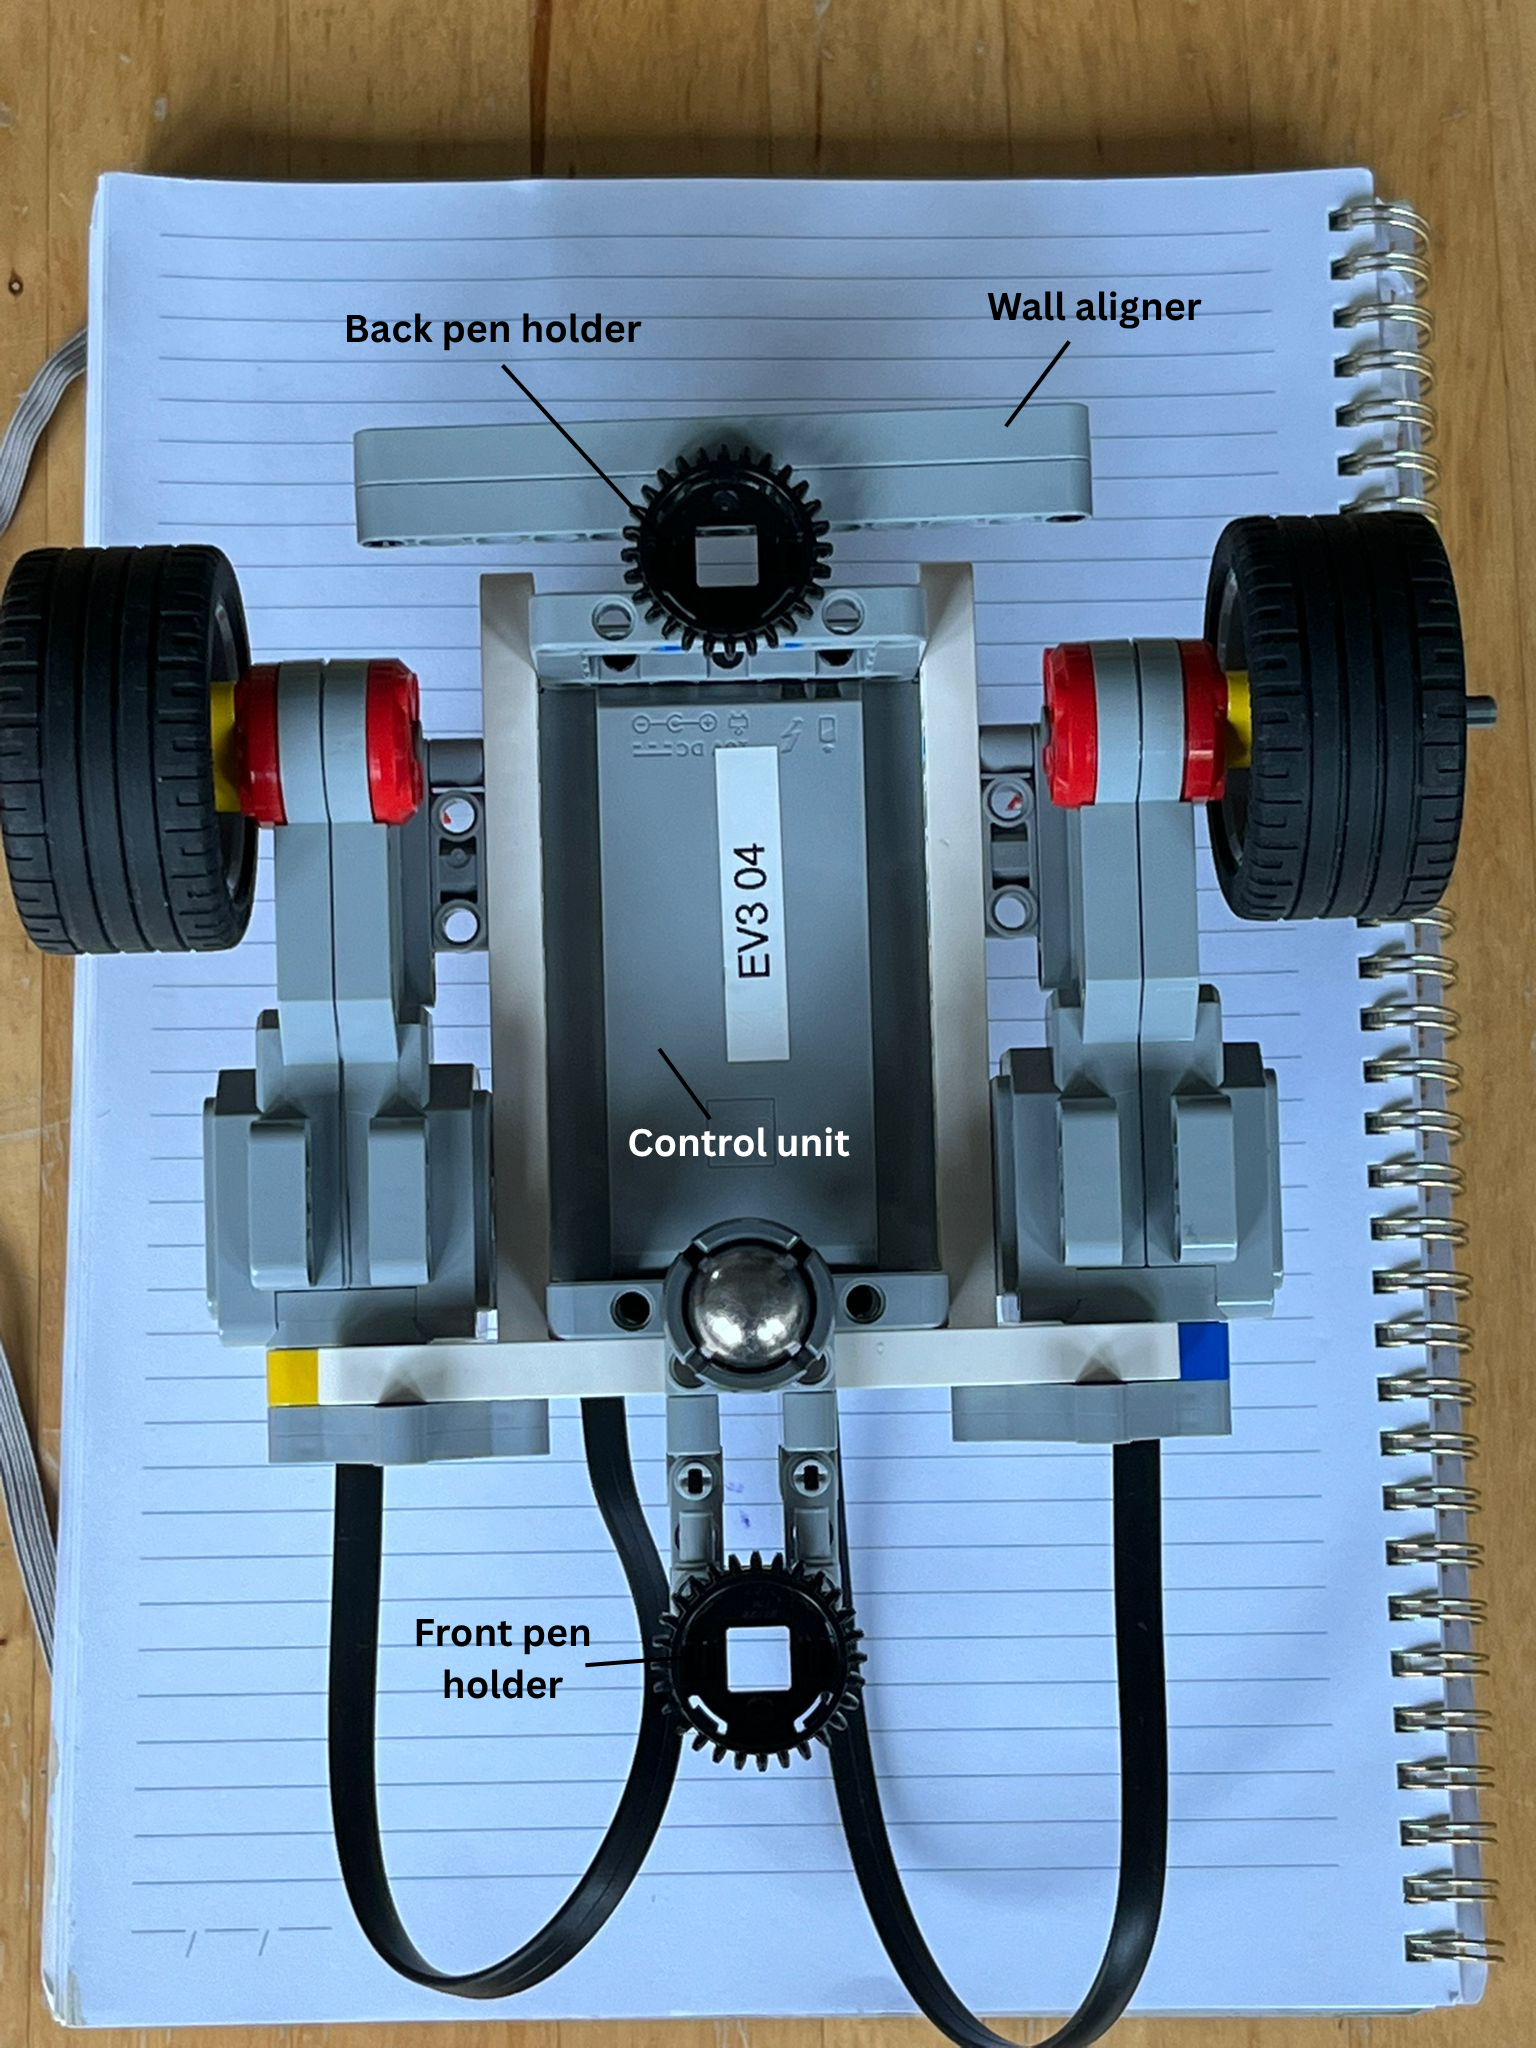
\includegraphics[width=0.8\linewidth]{figures/robot_angles/bottom.png}
        \caption{Top view of the robot}
        \label{fig:top_view}
    \end{figure} 

    \begin{figure}[ht]
        \centering
        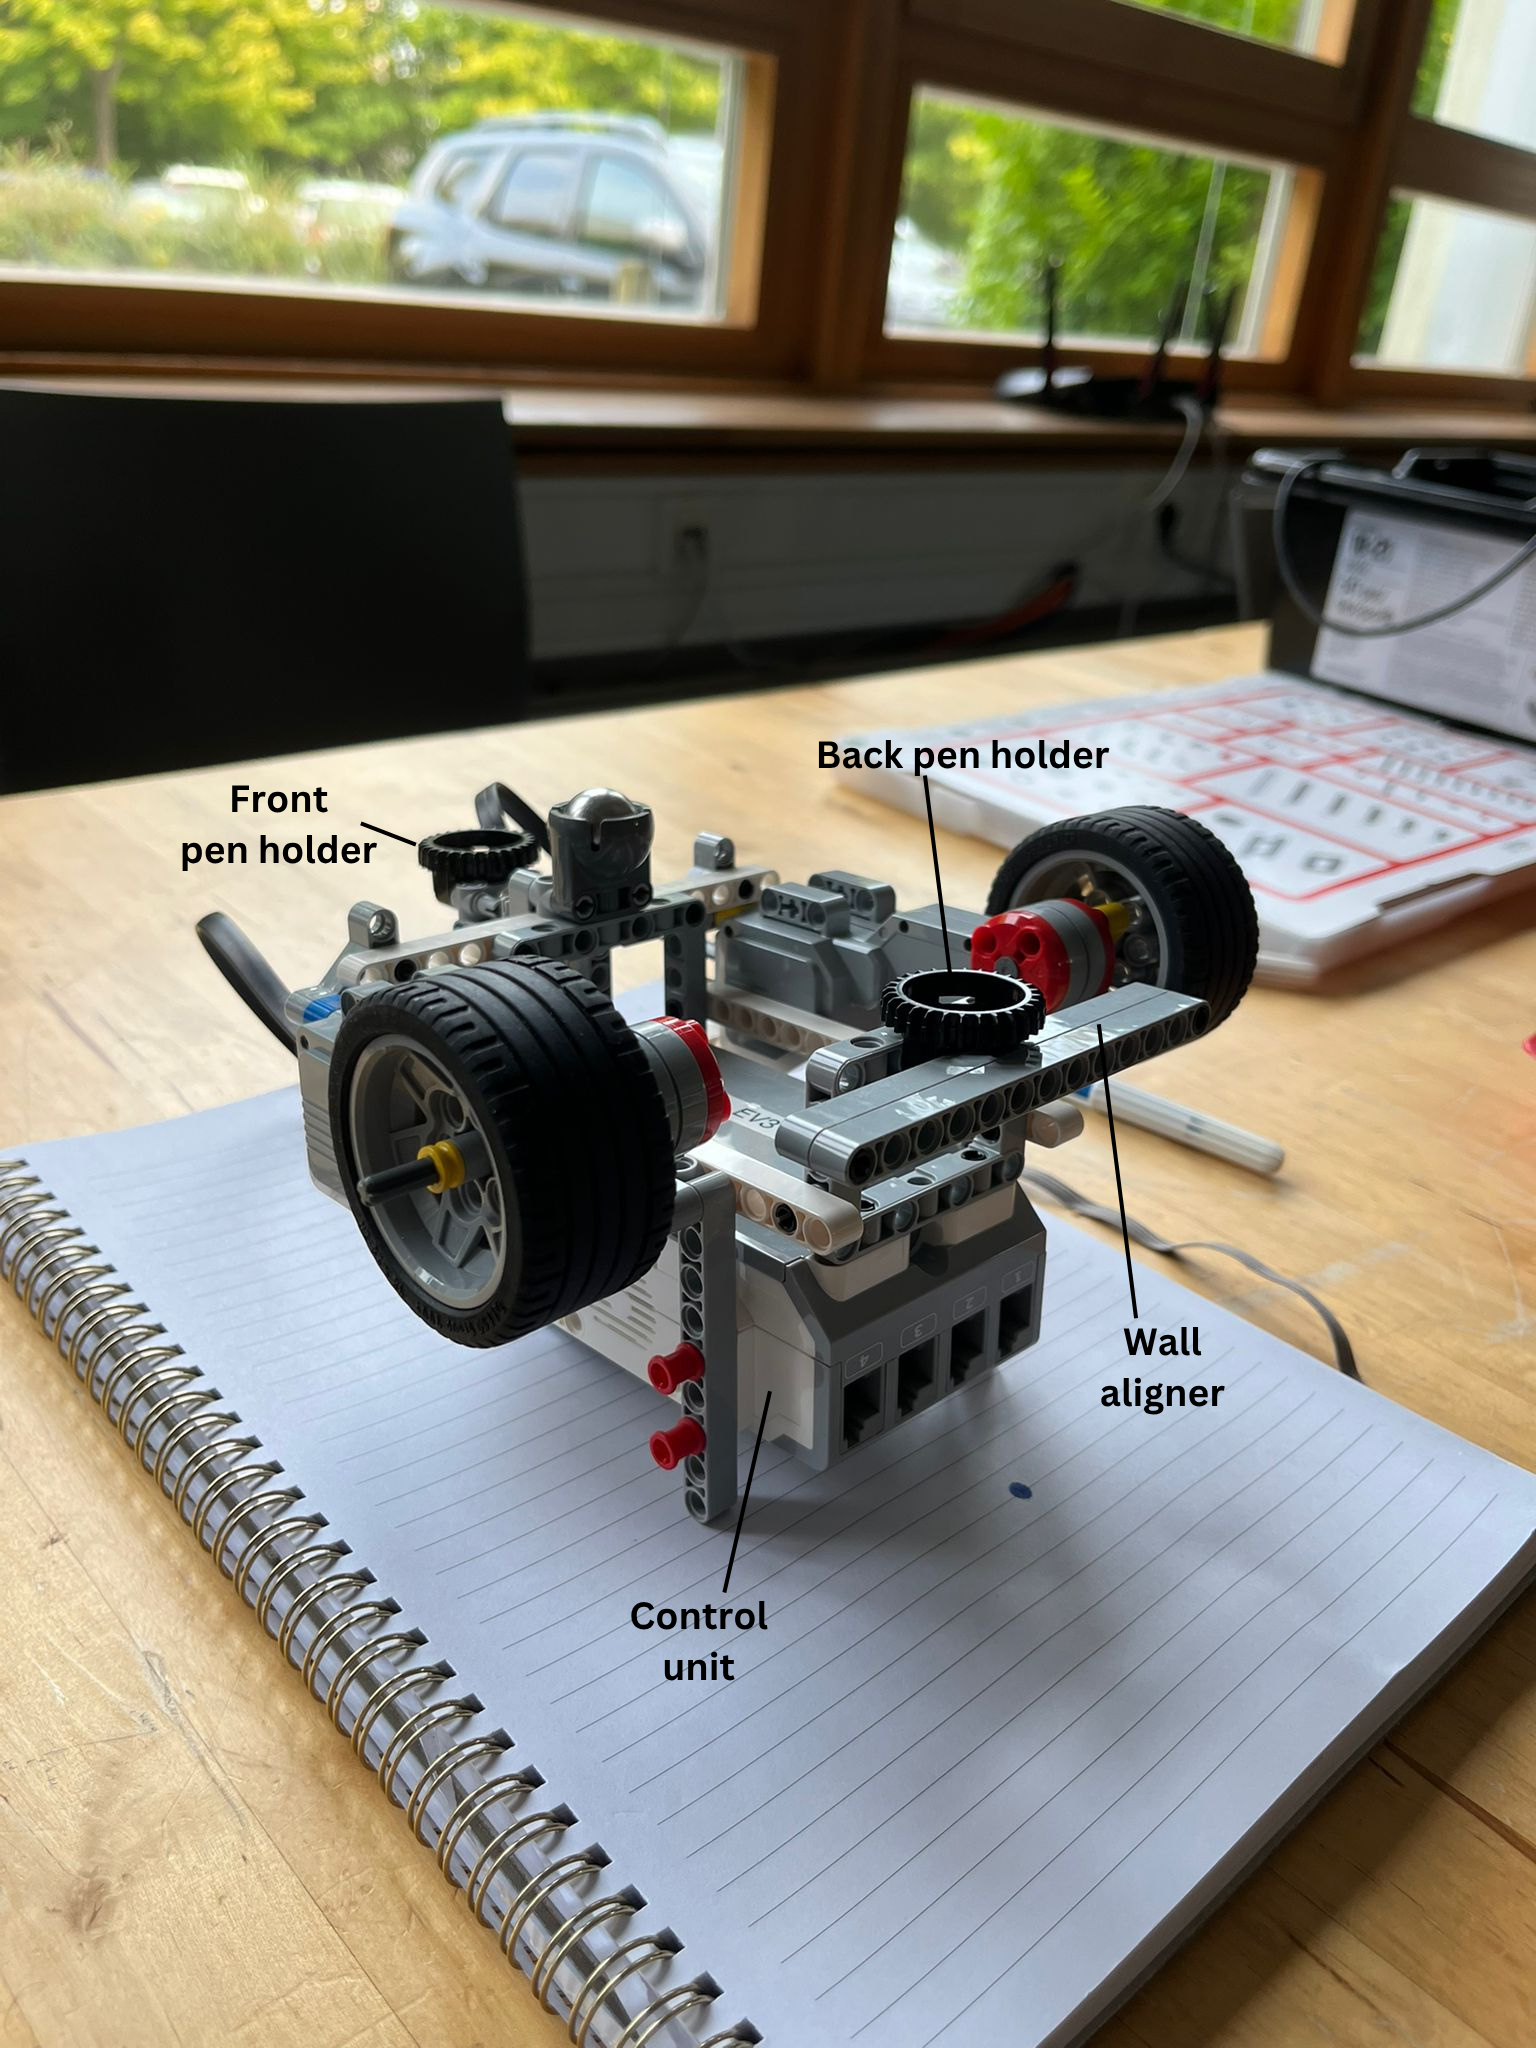
\includegraphics[width=0.8\linewidth]{figures/robot_angles/bottom_iso.png}
        \caption{Top view of the robot}
        \label{fig:top_view}
    \end{figure} 


\cite{referenceexample}

\subsection{Estimates of the expected Precision}
PUT ERROR DUE TO MEASUREING HERE

\subsection{Jacobian Error Propagation}

Let $\mathbf{F}$ be a vector function, defining the \textbf{end pose} of the robot, calculated from two measured positions on a 2D plane, $\mathbf{x}_1$ and $\mathbf{x}_2$. The output components are defined such that $\mathbf{F}_1$ and $\mathbf{F}_2$ represent the position coordinates and $\mathbf{F}_3$ represents the angle of the end pose. It is important to note that $\mathbf{F}_3$ can only be used if $x_{1,2} \neq x_{2,2}$, otherwise the orientation is either $\frac{\pi}{2}$ for $x_{1,1} > x_{2,1}$, or $-\frac{\pi}{2}$ for $x_{1,1} < x_{2,1}$ The input vectors and the functional relationship are defined in Equations \ref{eq:x1x2} to \ref{eq:F}.

\begin{eqnarray}
	\mathbf{x}_1 &=& \begin{pmatrix} x_{1,1} \\ x_{1,2} \end{pmatrix} \label{eq:x1x2} \\
	\mathbf{x}_2 &=& \begin{pmatrix} x_{2,1} \\ x_{2,2} \end{pmatrix} \\
	\mathbf{F}(\mathbf{x}_1, \mathbf{x}_2) &=& \begin{pmatrix}
		\frac{1}{2}(x_{1,1} + x_{2,1}) \\
		\frac{1}{2}(x_{1,2} + x_{2,2}) \\
		\arctan\left(\frac{x_{2,1}-x_{1,1}}{x_{2,2}-x_{2,1}}\right)
	\end{pmatrix} \label{eq:F}
\end{eqnarray}

The propagation of uncertainty in the measured input coordinates requires the calculation of the \textbf{Jacobian matrix} $\mathbf{J}$. The total input vector $\mathbf{x} = (x_{1,1}, x_{1,2}, x_{2,1}, x_{2,2})^T$ is composed of all four scalar variables. Since $\mathbf{F}$ is a vector-valued function with three outputs and four inputs, the resulting Jacobian matrix $\mathbf{J}$ is a $3 \times 4$ matrix, presented in Equations \ref{eq:Jac} to \ref{eq:Jac_end}.

\begin{eqnarray}
	\mathbf{J} &=& \frac{\partial \mathbf{F}}{\partial \mathbf{x}} =
	\begin{pmatrix}
		\frac{\partial F_1}{\partial x_{1,1}} & \frac{\partial F_1}{\partial x_{1,2}} & \frac{\partial F_1}{\partial x_{2,1}} & \frac{\partial F_1}{\partial x_{2,2}} \\
		\frac{\partial F_2}{\partial x_{1,1}} & \frac{\partial F_2}{\partial x_{1,2}} & \frac{\partial F_2}{\partial x_{2,1}} & \frac{\partial F_2}{\partial x_{2,2}} \\
		\frac{\partial F_3}{\partial x_{1,1}} & \frac{\partial F_3}{\partial x_{1,2}} & \frac{\partial F_3}{\partial x_{2,1}} & \frac{\partial F_3}{\partial x_{2,2}}
	\end{pmatrix} \label{eq:Jac} \\
	&=& \begin{pmatrix}
		\frac{1}{2}               & 0                         & \frac{1}{2}               & 0                         \\
		0                         & \frac{1}{2}               & 0                         & \frac{1}{2}               \\
		\frac{x_{1,2}-x_{2,2}}{d} & \frac{x_{2,1}-x_{1,1}}{d} & \frac{x_{2,2}-x_{1,2}}{d} & \frac{x_{1,1}-x_{2,1}}{d}
	\end{pmatrix} \\
	d &=& (x_{1,1}-x_{2,1})^2+(x_{1,2}-x_{2,2})^2 \label{eq:Jac_end}
\end{eqnarray}

The \textbf{covariance matrix of the calculated end pose}, $\mathbf{C}_F$, is then determined from the input covariance matrix, $\mathbf{C}_x$, via the generalized error propagation formula, which can be seen in Equation \ref{eq:CF}.

\begin{equation}
	\mathbf{C}_F = \mathbf{J} \, \mathbf{C}_x \, \mathbf{J}^T \label{eq:CF}
\end{equation}
where $\mathbf{C}_x$ is the $4 \times 4$ covariance matrix of the input variables $(x_{1,1}, x_{1,2}, x_{2,1}, x_{2,2})$.




\end{document}
